





Given $X$ and $Y$ are two independent random\\
variables. \\
Given $W=XI_{\{Y\leq X^2\}}$ \\
$X \in \brak{0,1}$ , $Y \in \brak{0,1}$ , $W \in [0,1)$\\
\begin{enumerate}
\item We need to find CDF of $W$
\begin{enumerate}
\item The PDF for $X$ is
\begin{align}
p_X(x) = 
\begin{cases}
     1 & 0 < x  < 1 \\
     0 & otherwise 
\end{cases}\label{june2013-70:1}
\end{align}
\item The CDF for $X$ is
\begin{align}
F_{X}(x)  = 
\begin{cases}
      0 & x \leq 0 \\
      x & 0 < x < 1 \\
      1 & otherwise
\end{cases}  \label{june2013-70:eq:2}
\end{align}
\item The PDF for $Y$ is
\begin{align}
p_{Y}(y)  = 
\begin{cases}
      1 & 0 < y < 1 \\
      0 & otherwise 
\end{cases} \label{june2013-70:3}
\end{align}
\item The CDF for $Y$ is
\begin{align}
F_{Y}(y)  = 
\begin{cases}
      0 & y \leq 0 \\
      y & 0 < y < 1 \\
      1 & otherwise 
\end{cases}\label{june2013-70:4}
\end{align}
\item $I_{\{Y\leq X^2\}}$ is defined as follows
\begin{align} 
I_{\{Y\leq X^2\}} =
\begin{cases}
    1 & y \leq x^2  \\
    0 & otherwise 
\end{cases} \label{june2013-70:5}
\end{align}
\item $W$ is defined as follows
\begin{align}
W  = 
\begin{cases}
    x & y \leq x^2 \\
    0 & otherwise
\end{cases}  \label{june2013-70:6}
\end{align}
From \eqref{june2013-70:6}
\begin{align}
p_W(W=0) &= \Pr(I_{\{Y\leq X^2\}}=0) \\
         &=\Pr(x^2 <y) \label{june2013-70:7}
\end{align}
\item Let $Z=X^2-Y$ be a random variable where $Z \in \brak{-1,1}$

\begin{align}
F_{X^2}(u)&=\Pr(X^2 \leq u) \\
          &=\Pr(X \leq \sqrt{u}) \\
          &=F_X(\sqrt{u}) \label{june2013-70:8}
\end{align}
\begin{enumerate}
\item From \eqref{june2013-70:eq:2},The CDF for $X^2$ is
\begin{align}
F_{X^2}(u)  = 
\begin{cases}
      0 & u \leq 0 \\
      \sqrt{u} & 0 < u < 1 \\
      1 & otherwise
\end{cases} \label{june2013-70:9}
\end{align}
\item The PDF for $X^2$ is
\begin{align}
p_{X^2}(u)  = 
\begin{cases}
      \frac{1}{2\sqrt{u}} & 0 < u < 1 \\
      0 & otherwise
\end{cases} \label{june2013-70:10}
\end{align}
\begin{align}
F_{\{-Y\}}(v)&=\Pr(-Y \leq v) \\
          &=\Pr(Y \geq -v) \\
          &=1-F_Y(-v) \label{june2013-70:11}
\end{align}
\item From \eqref{june2013-70:4},The CDF for $(-Y)$ is
\begin{align}
F_{\{-Y\}}(v)  = 
\begin{cases}
      0 & v \leq -1\\
      1+v & -1 < v < 0 \\
      1 & otherwise 
\end{cases}\label{june2013-70:12}
\end{align}
\item The PDF for $(-Y)$ is
\begin{align}
p_{\{-Y\}}(v)  = 
\begin{cases}
      1 & -1 < v < 0 \\
      0 & otherwise
\end{cases} \label{june2013-70:p-y}
\end{align}
\item $Z=X^2-Y$ $\implies  z=u+v$\\
Using convolution
\begin{align}
p_Z(z)=\int_{- \infty}^{\infty} p_{X^2}(z-v)p_{\{-Y\}}(v) \mathrm{dv} \label{june2013-70:pz}
\end{align}
Solving \eqref{june2013-70:pz} using \eqref{june2013-70:p-y},\eqref{june2013-70:10} for $z \in (-1,1)$, we get PDF of $Z$ as follows
\begin{align}
p_{Z}(z)  = 
\begin{cases}
      \sqrt{z+1} & -1 < z \leq 0 \\
      1-\sqrt{z} & 0 < z <1 \\
      0 & otherwise 
\end{cases} \label{june2013-70:13}
\end{align}
\item CDF of $Z$ as follows
\begin{align}
F_{Z}(z)  = 
\begin{cases}
      \frac{2}{3}{(z+1)}^\frac{3}{2} & -1 < z \leq 0 \\
      z-\frac{2}{3}{z}^\frac{3}{2} & 0 < z < 1 \\
      1 & otherwise
\end{cases} \label{june2013-70:14}
\end{align}

\end{enumerate}

\item using \eqref{june2013-70:14} to find $p_W(W=0)$
\begin{align}
p_W(W=0) &=\Pr(x^2 <y) \\
         &=F_z(0) \\
         &=\frac{2}{3} \label{june2013-70:15}
\end{align}

\item $W=t \implies X=t $ where $t \in (0,1)$
\begin{align}
p_{W}(t) = \int_{- \infty}^{\infty} p_X(t)I_{\{y\leq t^2\}} \mathrm{dy}
\end{align}
\begin{align}
   0 &< y < 1 \label{june2013-70:16} \\
   0 &< y \leq t^2  \label{june2013-70:17}
\end{align}
For $ 0 < t < 1 $,
\begin{align}
p_W(t) &= \int_{0}^{t^2} p_X(t)I_{\{y\leq t^2\}} \mathrm{dy} \\
       &= t^2 \label{june2013-70:18}
\end{align}
\item $\therefore$ PDF of $W$ is as follows
\begin{align}
p_{W}(t)  = 
\begin{cases}
  \frac{2}{3}& t=0 \\
  t^2 & 0 < t < 1 \\
  0 & otherwise
\end{cases} \label{june2013-70:19}
\end{align}
\item The CDF  of $W$ is as follows:
\begin{align}
F_W(t)  = 
\begin{cases}
  0 & t<0 \\
  \frac{2+t^3}{3}& 0 \leq t\leq 1\\
  1 & otherwise
\end{cases} \label{june2013-70:20}
\end{align}
\end{enumerate}
\item We need to find $P\sbrak{W>0}$
\begin{align}
\Pr(W > 0)&= 1- F_W(0) \\
           &=\frac{1}{3} \label{june2013-70:21} \\
\therefore \Pr(W>0)&=\frac{1}{3}
\end{align}
\item CDF of $W$ is discontinuous at $W=0$.\\
$\therefore$ option $3$ is incorrect.\\
\item The CDF in \eqref{june2013-70:20} can be written as
\begin{align}
  F_W(t)=\brak{\frac{2+t^3}{3}}I_{\{0\leq t \leq 1\}}+ I_{\{t > 1\}}
\end{align}
$\therefore$ option $2$ and $4$ are correct.
\begin{figure}[htb!]
\begin{center}
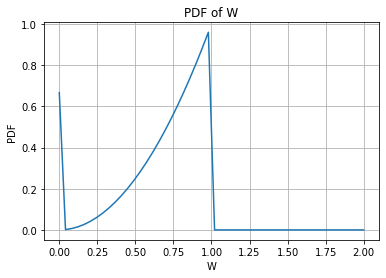
\includegraphics[width=\columnwidth]{solutions/2013/june/70/figures/assignment8pdf.png}
\end{center}
\end{figure}

\begin{figure}[htb!]
\begin{center}
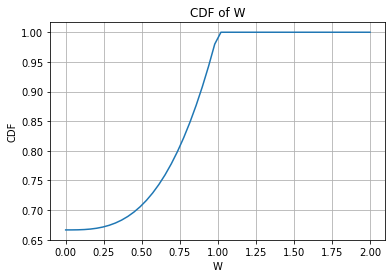
\includegraphics[width=\columnwidth]{solutions/2013/june/70/figures/assignment8cdf.png}
\end{center}
\end{figure}
\end{enumerate}
